\chapter{Introduction}

The internet as we know it today heavily relies on the use of the HTTP protocol. Not only is it used
by web browsers for interacting with websites, but it is also heavily used server-side for
communication between individual services, especially in the microservices architecture. HTTP is
also used as a transport medium for technologies such as gRPC and GraphQL\@. \todo{do I need
  citations for these techs?}

The latest version of the HTTP protocol is HTTP/2 published in 2015~\cite{rfc7540}. HTTP/2
improved on its predecessor HTTP/1.1~\cite{rfc7230} by introducing features such as request
multiplexing over a single TCP connection, header compression, and the server-push feature, allowing
it to significantly reduce loading times of web pages and generally improve the efficiency of the
web~\cite{deSaxce2015}.

\section{Performance Issues Remaining in HTTP/2}

However, HTTP/2 does not solve all performance issues HTTP/1.1 had. Some performance aspects of HTTP
can't be improved by changing the application layer of the HTTP protocol stack. For the context of
this thesis, the following two problems are most relevant.

\subsection*{Head-of-Line Blocking}

Request multiplexing was introduced in HTTP/2 to reduce the number of resources used by web servers
when serving requests made by web browsers. Because modern web pages are composed of many parts
(HTML, images, Javascript files, CSS style sheets), multiple HTTP requests have to be made to load
the page. In HTTP/1.1, multiple HTTP connections are made to download individual parts of the
webpage, one connection per HTTP request. In HTTP/2, a single connection can be used to make
multiple HTTP requests in parallel. Although this change improved the performance of HTTP, its
current design is limited by phenomenon generally known as \textit{head-of-line blocking}.

The individual HTTP frames which make up the HTTP requests are interleaved into a single stream of
data transferred over TCP connection. Because of TCP's guaranteed in-order delivery, loss of a
single packet will delay transmission of the following packets, and therefore all HTTP requests
currently in progress, even if the lost packet carried data for only one particular HTTP request.
More information on head-of-line blocking can be found e.g.\ on a dedicated Wikipedia
page~\cite{wiki:head-of-line_blocking}.

\subsection*{HTTPS Connection Establishment Latency}
HTTPS~\cite{rfc2818} is an extension to HTTP, which makes the connection encrypted by inserting the
TLS layer between HTTP and TCP\@. Establishing HTTPS connection, therefore, requires first
establishing TCP connection --- performing the three-way handshake --- and then performing another
separate handshake for the TLS layer. As can be seen on illustration in
figure~\ref{fig:https-packets}, a minimum of three round trips are needed before the HTTP request
can be sent.

\begin{figure}[h]
  \centering
  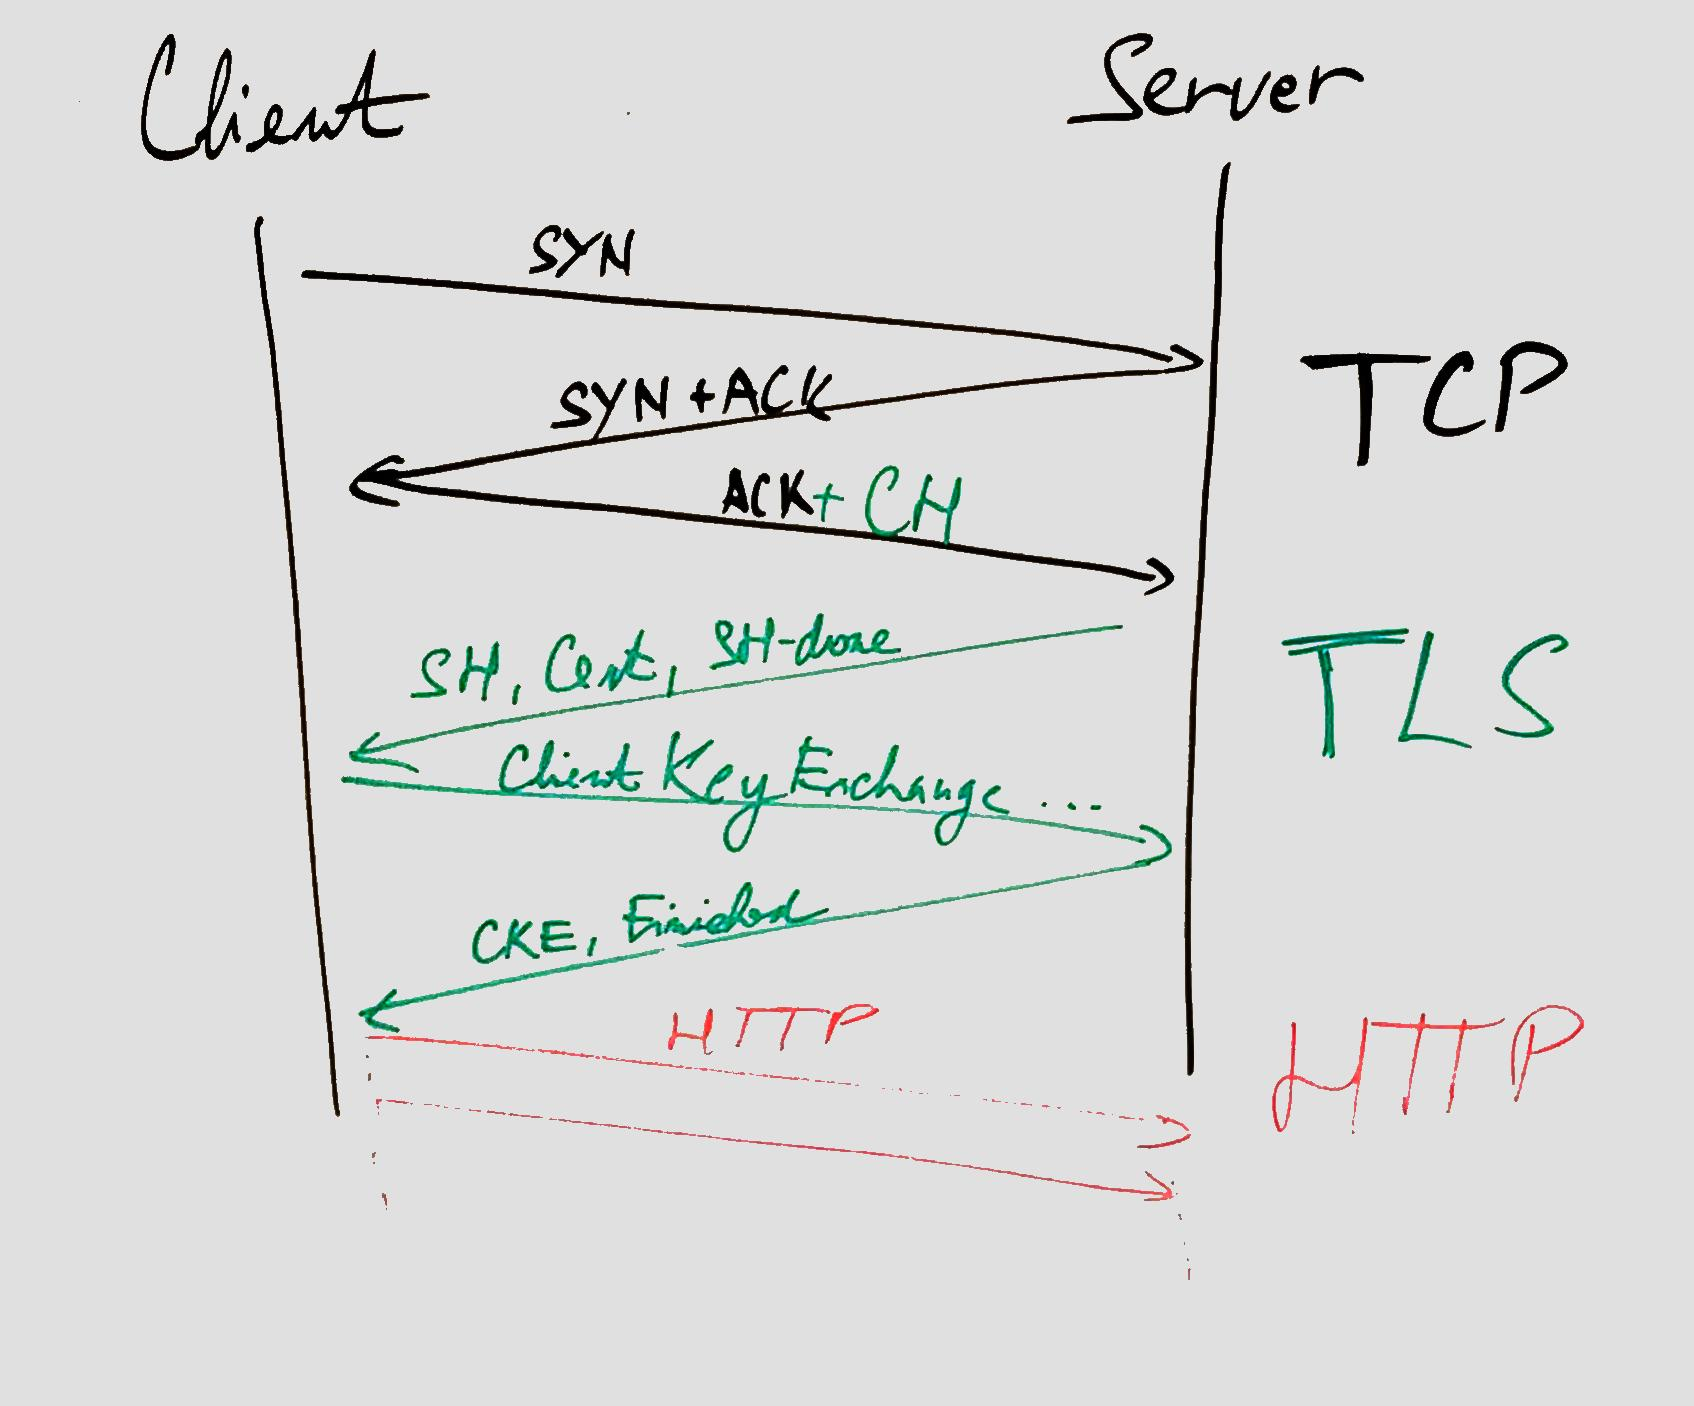
\includegraphics[width=0.6\textwidth]{img/01-https-connection-packets}
  \caption{Simplified view of the packets sent during HTTPS connection establishment}\label{fig:https-packets}
\end{figure}

To protect the privacy of their users, more and more websites enforce the use of HTTPS\@.
In August 2020, 96 out of the top 100 viewed websites actively redirect to HTTPS, and more than 75\%
of all network traffic from the Chrome web browser used HTTPS~\cite{googleTransparency}. With HTTPS
becoming the norm, almost all connections suffer from the increased latency caused by the
additional TLS handshake.

\section{HTTP/3 and QUIC}

The next version of the HTTP protocol --- HTTP/3~\cite{draft-ietf-quic-http-29} --- addresses the
above-mentioned issues by replacing the TCP and TLS layers with a brand new UDP-based protocol named
QUIC\footnote{Originally intended as the acronym for Quick UDP Internet Connection, but it has been
changed to be the actual name of the protocol during the standardization process}. The features of
the QUIC protocol allow moving responsibilities between layers of the HTTP protocol stack. The
responsibilities and relationships between protocols on HTTP/2 and HTTP/3 stacks are illustrated in
figure~\ref{fig:http2-vs-http3-stack}.

\begin{figure}[h]
  \centering
  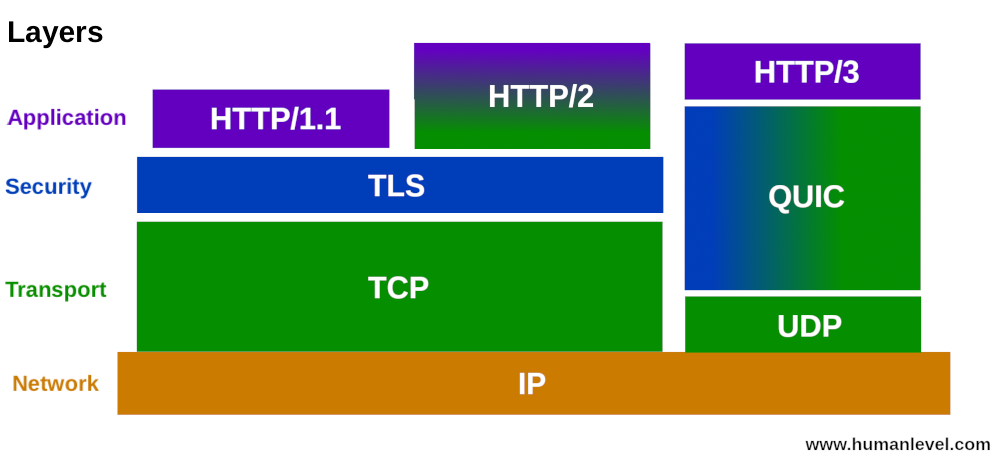
\includegraphics[width=\textwidth]{img/01-pile-http-protocol}
  \todo{Redraw this without HTTP/1.1 in inkscape, indicate which parts of the stack implement stream
    multiplexing, encryption, reliability, etc.}
  \caption{Comparison between HTTP/2 and HTTP/3 protocol stacks}\label{fig:http2-vs-http3-stack}
\end{figure}

\todo{possibly more comments on the figure will go here}

Although QUIC development is tied with that of HTTP/3, it is designed as a general-purpose transport
layer protocol that can be used for other application-layer protocols as well. The main improvements
of QUIC over TCP+TLS can be summarized in the following points:

\begin{itemize}
  \litem{Stream multiplexing} QUIC provides an abstraction of multiple streams of data multiplexed
    on a single connection. And because loss detection is implemented also at the QUIC layer, packet
    loss can be managed in a way that does not exhibit the head-of-line blocking problem described
    above.

  \litem{Faster connection establishment} QUIC also performs TLS 1.3 handshake, but it does so in
    parallel with the handshake for the base protocol. This combined handshake requires fewer
    round-trips and is, therefore, faster when compared to TCP+TLS\@.

    QUIC also supports opt-in TLS 1.3 Zero Round Trip Time Resumption (0-RTT for short). The 0-RTT
    mode of operation allows a client to cache some session information allowing it to send
    application data with the very first packet in future connection to the same server. This
    effectively reduces the latency by another round trip but makes such requests vulnerable to
    repeat attacks. A more detailed description of 0-RTT can be found online, e.g.\ on Cloudflare's
    blog~\cite{cloudflare-0rtt}.

  \litem{Always encrypted} TLS handshake is a mandatory part of connection establishment and
    encryption, therefore, cannot be turned off. This makes QUIC secure-by-default.

  \litem{Separating connection identity from peer's IP address} QUIC protocol does not use peers
    IP addresses to identify connections but instead uses connection IDs which are 8 to 20-byte
    sequences negotiated during connection establishment.

    This makes QUIC very attractive for mobile devices, which can switch between multiple IP
    addresses. This happens e.g.\ when the device switches from Wi-Fi to a cellular data network.
    Ordinarily, the existing connection has to be terminated and a new connection established from
    the new IP address. QUIC, on the other hand, can migrate the connections in a way that is
    transparent to the application layer.

    This feature also enables QUIC extensions like Multipath
    QUIC~\cite{draft-deconinck-quic-multipath-04}, which allows the simultaneous use of multiple
    network interfaces for a single connection to achieve greater throughput.

\end{itemize}

As of August 2020, the specifications of HTTP/3 and QUIC are still at the draft stage, but the
standardization process is believed to be very close to complete. There are already multiple
implementations of the draft versions of the standard and many of these implementations are backed
by big companies such as Google, Cloudflare, Facebook, and Microsoft.

Experiments with these implementations allow early performance comparison between HTTP/3 and HTTP/2.
In 2015 the experimental implementation by the Chromium team showed a 3\% improvement in mean page
load time and 30\% fewer rebuffer events when watching YouTube videos~\cite{Wilk2015}. Cloudflare
launched preliminary support for HTTP/3 in April 2020 and has measured a 12.4\% decrease in the
\textit{time to the first byte} metric~\cite{Tellakula2020}, which is consistent with the QUICs
promise of reduced latency. The QUIC protocol outperforms TCP especially in unstable networks such
as wireless mobile networks~\cite{Cook2017}.

\section{Support for QUIC in \dotnet{}}

Microsoft's \dotnet{} development team has long-term plans to provide full QUIC and HTTP/3 support
in \dotnet{}. In the case of HTTP/3, the support should be completely transparent to users, because
the implementation of \texttt{HttpClient} automatically chooses the best available HTTP
version~\cite{HttpClientDocs}. Since QUIC can be used to build other protocols than HTTP/3, its
implementation will be exposed via public classes residing most likely inside the
\texttt{System.Net.Quic} namespace.

The QUIC support has been originally intended for the \dotnet{} 5 release planned for November 2020.
However, it turned out that the standardization process wasn't going to be completed in time for
QUIC to be implemented for the release, so the work was interrupted and official HTTP/3 and QUIC
support was postponed for later releases.

\todo{probably remove the following subsection heading}

\subsection*{Existing QUIC Implementation in \dotnet{}}

The work-in-progress implementation of QUIC is still present in the master development branch of the
\dotnet{} runtime repository~\cite{dotnetGithub} but has been made accessible only internally. This
implementation is a wrapper around the \libmsquic{} library~\cite{msquicGithub}, which is a C
implementation of QUIC developed by Microsoft. The \libmsquic{} library is designed for
high-performance scenarios and has been recently open-sourced.

The decision to use \libmsquic{} as the QUIC protocol implementation is not final. Using an existing
external implementation allows the development team to quickly evaluate the proposed QUIC API\@.
However, there are compelling arguments for implementing the QUIC protocol in managed \dotnet{} code
--- and more specifically, in \csharp{} --- for the production release.

The existing QUIC implementation in \dotnet{} uses a layer of indirection which allows multiple
implementations to exist side by side. In theory, this makes it possible to switch between QUIC
implementations at runtime, which can be used to compare the performance between different QUIC
implementations.

% It is also cross-platform, with support for Windows and Linux operating systems.

\subsection*{Motivation for Implementing QUIC in Managed Code}

Code written in ahead-of-time compiled languages such as C or C++ (from now on referred to as
\textit{native code}) is likely to be faster than code written in \dotnet{} languages (from now on
referred to as \textit{managed code}), which rely on the just-in-time compilation. However, there
are other aspects than raw performance to be considered when deciding to use native libraries such
as \libmsquic{}:

\begin{itemize}

  \litem{Cross-platform compatibility/availability} The \dotnet{} platform officially supports
    multiple versions of Windows, macOS, and several Linux distributions. If the native library does
    not support all these platforms, then an alternative library has to be used on other platforms,
    introducing more complexity into the codebase.

  \litem{Support for different library versions} Currently, no native libraries that managed
    \dotnet{} libraries depend on are part of the \dotnet{} distribution. Instead, it is expected
    that the library is already installed on the target machine and can be dynamically loaded. This
    means that the \dotnet{} code must work correctly with multiple different versions of the native
    library.

  \litem{Maintainability} Maintenance of the interop code requires the developer to be able to
    read and understand the language in which the native library is written. Debugging the code
    around the language boundaries can be difficult in case the necessary tooling for mixed-language
    debugging is not available.

  \litem{Library's API} One of the aspects which greatly influences the resulting performance is
    the similarity between the public API of the \dotnet{} library and the API of the native
    library. Some aspects are the following:

    \begin{itemize}
      \item Event-based (using callbacks) vs.\ method based
      \item Blocking vs.\ non-blocking
      \item Synchronous vs.\ asynchronous
      \item Which side allocates memory buffers
    \end{itemize}

    Managed code needs to translate the differences between APIs, which may result in noticeable
    performance overhead and even negate the performance gained from the use of the native library.

  \litem{Overhead of native calls} \todo{cost of pinvoke call}

  \litem{Future development} Exposing new features from newer versions of the native library can
    be problematic because the code needs to work also with older versions of the library.

\end{itemize}

In the past, the \dotnet{} development team has encountered multiple problems with the
\libcurl~\cite{curlGithub} library, which was used to implement HTTP request handling \todo{On linux
  only?}. Different
Linux distributions contain different versions of the \libcurl{} library supporting different
features and having different bugs. The \dotnet{} development team had to expend a lot of resources to make sure
the managed code written by other \dotnet{} developers behaved consistently on all platforms.

Starting with \dotnet{} Core 2.1, the default implementation of HTTP request handling does not rely
on native libraries like \libcurl{}. Instead, the functionality has been rewritten in pure managed
code, which offered better performance and consistent behavior across all \dotnet{}
platforms~\cite{SocketsHttpHandlerDocs}.

\section{Goals of this Thesis}

The reasons mentioned in the previous section motivated Microsoft developers to consider
implementing QUIC in purely managed \csharp{} code. Before the final decision which implementation
of QUIC will be used, it is necessary to investigate the actual performance characteristics of
managed QUIC implementation. This thesis seeks to create a partial implementation of QUIC, which
should aid in this decision.

Because the work of this thesis can become the basis of the future QUIC implementation in the
following \dotnet{} 6 release, the development of the QUIC implementation will occur inside a
development branch of the \dotnet{} runtime repository. The result should be a compilable branch of
the runtime, which exposes the QUIC API for other \dotnet{} developers to use.

We have mentioned that the design of the QUIC API was interrupted early. Although the current
version does not expose all features of the QUIC protocol, it is sufficient for evaluating of our
implementation. This thesis will, therefore, avoid making any modifications to the API\@.

\todo{I think this paragraph should be completely removed and moved to the analysis chapter.}
Although the managed QUIC implementation should be portable, the API necessary for integrating TLS
into QUIC is currently unavailable in the native libraries used by \dotnet{}. To avoid implementing
TLS 1.3 ourselves, this thesis will select a suitable TLS library and integrate it into the QUIC
implementation. Dependence on another library is expected to be temporary until the QUIC enabling
APIs are present in TLS libraries currently in use in \dotnet{}.

Implementing the full QUIC specification is outside the scope of a master thesis. Fortunately, to
evaluate the performance of the managed QUIC implementation, many of the parts of the specification
can be omitted from our prototype. This thesis will, therefore, focus on the functionality needed to
fully support simple scenarios and will leave out features such as connection migration.

Because we do not expect readers to be fully familiar with the QUIC protocol specification and all
its features, we will present an overview of the protocol in Chapter~\ref{chap:02-quic} and defer
selection of the protocol features to be implemented as part of this thesis to the beginning of the
analysis in Chapter~\ref{chap:03-analysis}. The design of the implementation, however, should be
such that the rest of the specification can be implemented in the future.

It would make sense to evaluate the functionality of our QUIC implementation by providing also a
partial implementation of HTTP/3. However, even supporting the simplest GET requests would be too
complex. Instead, we will implement a primitive client-server console application. The client part
of the application will send all files in a given directory to the server, which will store them in
a directory. The files will be sent in parallel, utilizing the stream multiplexing feature of
QUIC\@.

In the previous section we mentioned that the indirect nature of the existing QUIC API can be used
to alternate between \libmsquic{}-based QUIC and our QUIC implementation at runtime. As an optional
goal, this thesis will use this to compare the performance characteristics between these two
implementations and compare these to performance to that of TCP+TLS based \texttt{SslStream}.

\subsection*{Summary of the Goals}

The following list summarizes the goals of this thesis presented in the previous subsection.

\begin{enumerate}

  \item Select a sufficient subset of QUIC specification needed to support the most basic data
    transfer and implement it inside \dotnet{} runtime codebase.

  \item Expose the existing QUIC API, and allow switching between the new managed implementation and
    the existing \libmsquic{} based one.

  \item Evaluate the QUIC implementation by using it to implement a simple client-server console
    application for sending files.

  \item \todo{Emphasise that this is optional?} Try to compare the performance of the new
    implementation with the previous \libmsquic{}-based one.

\end{enumerate}
